
% This LaTeX was auto-generated from MATLAB code.
% To make changes, update the MATLAB code and republish this document.

\documentclass{article}
\usepackage{graphicx}
\usepackage{color}

\sloppy
\definecolor{lightgray}{gray}{0.5}
\setlength{\parindent}{0pt}

\begin{document}

    
    
\subsection*{Contents}

\begin{itemize}
\setlength{\itemsep}{-1ex}
   \item Fix parameters
   \item Export geometry
   \item Define the problem
   \item Generate the mesh
   \item Obtain relative matrices
   \item Assign true solution
   \item Iterations
   \item Plot of \texttt{\ensuremath{|}u\_n-u\_true}\ensuremath{|} versus Nsteps
\end{itemize}


\subsection*{Fix parameters}

\begin{verbatim}
tic;
Nsteps = 80;   % Number of iterations
Nplot = 101;   % Fineness of plots
T = 10*eps;   % Time delay
az = 13;      % Plot viewing angle
el = 48;      % Plot viewing height
v = 0.0;      % Camera speed
fix_axes = 0;               % Set to 1 for fixed axes
plot_range = [-0.1 1.1];    % z-axis range if fixed
% col_range = plot_range;   % Fixed colour range
% col_range = [-.7 1.1];
col_range = 'manual';       % Varying colour range
rec = 0;                    % record on/off
xg = linspace(-1,1,Nplot);
yg = linspace(-1,1,Nplot);
[XX,YY] = meshgrid(xg,yg);
ZZ = NaN(size(XX));

[indy_up,indx_up]=find(XX>=0);
indx_up = unique(indx_up);
indy_up = unique(indy_up);

[indy_lo,indx_lo]=find(YY<=0);
indx_lo = unique(indx_lo);
indy_lo = unique(indy_lo);

indices_all=find(XX>=0|YY<=0);
ZZ(indices_all)=1;
Du_dy=(ZZ(1:Nplot-2,:)-ZZ(3:Nplot,:));
Du_dx=(ZZ(:,3:Nplot)-ZZ(:,1:Nplot-2));
diffy_ind=~isnan(Du_dy);
diffx_ind=~isnan(Du_dx);
\end{verbatim}


\subsection*{Export geometry}

\begin{verbatim}
load('upper_rectangle')
load('lower_rectangle')
\end{verbatim}


\subsection*{Define the problem}

\begin{verbatim}
a = 1;
c = 1;        % Coeffs in PDE
f = 1;        % RHS of PDE
% f = '1+x.^2+12*(y+1)';
% f = '1./(x.^2+(y+1/2).^2)-1./((x-1/2).^2+y.^2)';

initguess=@(x,y) abs(log(1./((x.^2+y.^2).^.5))).^0.4999 % u0=infinity
% initguess=@(x,y) 1;
% initguess = @(x,y) 0; % u0~=1 @(0,0)
% initguess = @(x,y) -1-sin(22*x).*sin(10*y);
% initguess = @(x,y) 1-sin(22*x).*sin(10*y);
% initguess = @(x,y) 0.0+(min(x.^2+(y+.5).^2,(x-.5).^2+y.^2)<.005);
% initguess = @(x,y) (min(x.^2+(y+.5).^2,(x-.5).^2+y.^2)>.05);
% initguess = @(x,y) -3+4*(x.^2+(y+1/2).^2>.001);
% initguess = @(x,y) 1-.001./(x.^2+(y+1/2).^2).^(1/3)-.001./((x-1/2).^2+y.^2).^(1/3);
%initguess = @(x,y) 10-7.*(abs(log(-x.^2-(y+1/2).^2))).^0.4999;
\end{verbatim}

        \color{lightgray} \begin{verbatim}
initguess =

  function_handle with value:

    @(x,y)abs(log(1./((x.^2+y.^2).^.5))).^0.4999

\end{verbatim} \color{black}
    

\subsection*{Generate the mesh}

\begin{verbatim}
errvals_inf= zeros(4,Nsteps);
errvals_H1=zeros(4,Nsteps);

for Nmesh=25:25:100;
\end{verbatim}
\begin{verbatim}
meshgenfun = '1./(x.^2+y.^2)'; % function for adaptive mesh generation
[~,p_up,e_up,t_up]=adaptmesh(g_up,b_up,c,a,meshgenfun,'Ngen', Nmesh);
[~,p_lo,e_lo,t_lo]=adaptmesh(g_lo,b_lo,c,a,meshgenfun,'Ngen', Nmesh);
figure(1);
pdemesh(p_up,e_up,t_up);
xlim ([-1.5,1.5]);
axis equal;

figure(2);
pdemesh(p_lo,e_lo,t_lo);
xlim ([-1.5,1.5]);
axis equal;
\end{verbatim}

        \color{lightgray} \begin{verbatim}Number of triangles: 172
Number of triangles: 178
Number of triangles: 197
Number of triangles: 201
Number of triangles: 213
Number of triangles: 217
Number of triangles: 229
Number of triangles: 233
Number of triangles: 245
Number of triangles: 249
Number of triangles: 261
Number of triangles: 265
Number of triangles: 277
Number of triangles: 281
Number of triangles: 293
Number of triangles: 297
Number of triangles: 309
Number of triangles: 313
Number of triangles: 325
Number of triangles: 329
Number of triangles: 341
Number of triangles: 345
Number of triangles: 357
Number of triangles: 361
Number of triangles: 373
Number of triangles: 377

Maximum number of refinement passes obtained.
Number of triangles: 168
Number of triangles: 174
Number of triangles: 192
Number of triangles: 196
Number of triangles: 212
Number of triangles: 216
Number of triangles: 228
Number of triangles: 232
Number of triangles: 244
Number of triangles: 248
Number of triangles: 260
Number of triangles: 264
Number of triangles: 276
Number of triangles: 280
Number of triangles: 292
Number of triangles: 296
Number of triangles: 308
Number of triangles: 312
Number of triangles: 324
Number of triangles: 328
Number of triangles: 340
Number of triangles: 344
Number of triangles: 356
Number of triangles: 360
Number of triangles: 372
Number of triangles: 376

Maximum number of refinement passes obtained.
\end{verbatim} \color{black}
    
        \color{lightgray} \begin{verbatim}Number of triangles: 172
Number of triangles: 178
Number of triangles: 197
Number of triangles: 201
Number of triangles: 213
Number of triangles: 217
Number of triangles: 229
Number of triangles: 233
Number of triangles: 245
Number of triangles: 249
Number of triangles: 261
Number of triangles: 265
Number of triangles: 277
Number of triangles: 281
Number of triangles: 293
Number of triangles: 297
Number of triangles: 309
Number of triangles: 313
Number of triangles: 325
Number of triangles: 329
Number of triangles: 341
Number of triangles: 345
Number of triangles: 357
Number of triangles: 361
Number of triangles: 373
Number of triangles: 377
Number of triangles: 389
Number of triangles: 393
Number of triangles: 405
Number of triangles: 409
Number of triangles: 421
Number of triangles: 425
Number of triangles: 437
Number of triangles: 441
Number of triangles: 453
Number of triangles: 457
Number of triangles: 469
Number of triangles: 473
Number of triangles: 485
Number of triangles: 489
Number of triangles: 501
Number of triangles: 505
Number of triangles: 517
Number of triangles: 521
Number of triangles: 533
Number of triangles: 537
Number of triangles: 549
Number of triangles: 553
Number of triangles: 565
Number of triangles: 569
Number of triangles: 581

Maximum number of refinement passes obtained.
Number of triangles: 168
Number of triangles: 174
Number of triangles: 192
Number of triangles: 196
Number of triangles: 212
Number of triangles: 216
Number of triangles: 228
Number of triangles: 232
Number of triangles: 244
Number of triangles: 248
Number of triangles: 260
Number of triangles: 264
Number of triangles: 276
Number of triangles: 280
Number of triangles: 292
Number of triangles: 296
Number of triangles: 308
Number of triangles: 312
Number of triangles: 324
Number of triangles: 328
Number of triangles: 340
Number of triangles: 344
Number of triangles: 356
Number of triangles: 360
Number of triangles: 372
Number of triangles: 376
Number of triangles: 388
Number of triangles: 392
Number of triangles: 404
Number of triangles: 408
Number of triangles: 420
Number of triangles: 424
Number of triangles: 436
Number of triangles: 440
Number of triangles: 452
Number of triangles: 456
Number of triangles: 468
Number of triangles: 472
Number of triangles: 484
Number of triangles: 488
Number of triangles: 500
Number of triangles: 504
Number of triangles: 516
Number of triangles: 520
Number of triangles: 532
Number of triangles: 536
Number of triangles: 548
Number of triangles: 552
Number of triangles: 564
Number of triangles: 568
Number of triangles: 580

Maximum number of refinement passes obtained.
\end{verbatim} \color{black}
    
        \color{lightgray} \begin{verbatim}Number of triangles: 172
Number of triangles: 178
Number of triangles: 197
Number of triangles: 201
Number of triangles: 213
Number of triangles: 217
Number of triangles: 229
Number of triangles: 233
Number of triangles: 245
Number of triangles: 249
Number of triangles: 261
Number of triangles: 265
Number of triangles: 277
Number of triangles: 281
Number of triangles: 293
Number of triangles: 297
Number of triangles: 309
Number of triangles: 313
Number of triangles: 325
Number of triangles: 329
Number of triangles: 341
Number of triangles: 345
Number of triangles: 357
Number of triangles: 361
Number of triangles: 373
Number of triangles: 377
Number of triangles: 389
Number of triangles: 393
Number of triangles: 405
Number of triangles: 409
Number of triangles: 421
Number of triangles: 425
Number of triangles: 437
Number of triangles: 441
Number of triangles: 453
Number of triangles: 457
Number of triangles: 469
Number of triangles: 473
Number of triangles: 485
Number of triangles: 489
Number of triangles: 501
Number of triangles: 505
Number of triangles: 517
Number of triangles: 521
Number of triangles: 533
Number of triangles: 537
Number of triangles: 549
Number of triangles: 553
Number of triangles: 565
Number of triangles: 569
Number of triangles: 581
Number of triangles: 585
Number of triangles: 597
Number of triangles: 601
Number of triangles: 613
Number of triangles: 617
Number of triangles: 629
Number of triangles: 633
Number of triangles: 645
Number of triangles: 649
Number of triangles: 661
Number of triangles: 665
Number of triangles: 677
Number of triangles: 681
Number of triangles: 693
Number of triangles: 697
Number of triangles: 709
Number of triangles: 713
Number of triangles: 725
Number of triangles: 729
Number of triangles: 741
Number of triangles: 745
Number of triangles: 757
Number of triangles: 761
Number of triangles: 773
Number of triangles: 777

Maximum number of refinement passes obtained.
Number of triangles: 168
Number of triangles: 174
Number of triangles: 192
Number of triangles: 196
Number of triangles: 212
Number of triangles: 216
Number of triangles: 228
Number of triangles: 232
Number of triangles: 244
Number of triangles: 248
Number of triangles: 260
Number of triangles: 264
Number of triangles: 276
Number of triangles: 280
Number of triangles: 292
Number of triangles: 296
Number of triangles: 308
Number of triangles: 312
Number of triangles: 324
Number of triangles: 328
Number of triangles: 340
Number of triangles: 344
Number of triangles: 356
Number of triangles: 360
Number of triangles: 372
Number of triangles: 376
Number of triangles: 388
Number of triangles: 392
Number of triangles: 404
Number of triangles: 408
Number of triangles: 420
Number of triangles: 424
Number of triangles: 436
Number of triangles: 440
Number of triangles: 452
Number of triangles: 456
Number of triangles: 468
Number of triangles: 472
Number of triangles: 484
Number of triangles: 488
Number of triangles: 500
Number of triangles: 504
Number of triangles: 516
Number of triangles: 520
Number of triangles: 532
Number of triangles: 536
Number of triangles: 548
Number of triangles: 552
Number of triangles: 564
Number of triangles: 568
Number of triangles: 580
Number of triangles: 584
Number of triangles: 596
Number of triangles: 600
Number of triangles: 612
Number of triangles: 616
Number of triangles: 628
Number of triangles: 632
Number of triangles: 644
Number of triangles: 648
Number of triangles: 660
Number of triangles: 664
Number of triangles: 676
Number of triangles: 680
Number of triangles: 692
Number of triangles: 696
Number of triangles: 708
Number of triangles: 712
Number of triangles: 724
Number of triangles: 728
Number of triangles: 740
Number of triangles: 744
Number of triangles: 756
Number of triangles: 760
Number of triangles: 772
Number of triangles: 776

Maximum number of refinement passes obtained.
\end{verbatim} \color{black}
    
        \color{lightgray} \begin{verbatim}Number of triangles: 172
Number of triangles: 178
Number of triangles: 197
Number of triangles: 201
Number of triangles: 213
Number of triangles: 217
Number of triangles: 229
Number of triangles: 233
Number of triangles: 245
Number of triangles: 249
Number of triangles: 261
Number of triangles: 265
Number of triangles: 277
Number of triangles: 281
Number of triangles: 293
Number of triangles: 297
Number of triangles: 309
Number of triangles: 313
Number of triangles: 325
Number of triangles: 329
Number of triangles: 341
Number of triangles: 345
Number of triangles: 357
Number of triangles: 361
Number of triangles: 373
Number of triangles: 377
Number of triangles: 389
Number of triangles: 393
Number of triangles: 405
Number of triangles: 409
Number of triangles: 421
Number of triangles: 425
Number of triangles: 437
Number of triangles: 441
Number of triangles: 453
Number of triangles: 457
Number of triangles: 469
Number of triangles: 473
Number of triangles: 485
Number of triangles: 489
Number of triangles: 501
Number of triangles: 505
Number of triangles: 517
Number of triangles: 521
Number of triangles: 533
Number of triangles: 537
Number of triangles: 549
Number of triangles: 553
Number of triangles: 565
Number of triangles: 569
Number of triangles: 581
Number of triangles: 585
Number of triangles: 597
Number of triangles: 601
Number of triangles: 613
Number of triangles: 617
Number of triangles: 629
Number of triangles: 633
Number of triangles: 645
Number of triangles: 649
Number of triangles: 661
Number of triangles: 665
Number of triangles: 677
Number of triangles: 681
Number of triangles: 693
Number of triangles: 697
Number of triangles: 709
Number of triangles: 713
Number of triangles: 725
Number of triangles: 729
Number of triangles: 741
Number of triangles: 745
Number of triangles: 757
Number of triangles: 761
Number of triangles: 773
Number of triangles: 777
Number of triangles: 789
Number of triangles: 793
Number of triangles: 805
Number of triangles: 809
Number of triangles: 821
Number of triangles: 825
Number of triangles: 837
Number of triangles: 841
Number of triangles: 853
Number of triangles: 857
Number of triangles: 869
Number of triangles: 873
Number of triangles: 885
Number of triangles: 889
Number of triangles: 901
Number of triangles: 905
Number of triangles: 917
Number of triangles: 921
Number of triangles: 933
Number of triangles: 937
Number of triangles: 949
Number of triangles: 953
Number of triangles: 965
Number of triangles: 969
Number of triangles: 981

Maximum number of refinement passes obtained.
Number of triangles: 168
Number of triangles: 174
Number of triangles: 192
Number of triangles: 196
Number of triangles: 212
Number of triangles: 216
Number of triangles: 228
Number of triangles: 232
Number of triangles: 244
Number of triangles: 248
Number of triangles: 260
Number of triangles: 264
Number of triangles: 276
Number of triangles: 280
Number of triangles: 292
Number of triangles: 296
Number of triangles: 308
Number of triangles: 312
Number of triangles: 324
Number of triangles: 328
Number of triangles: 340
Number of triangles: 344
Number of triangles: 356
Number of triangles: 360
Number of triangles: 372
Number of triangles: 376
Number of triangles: 388
Number of triangles: 392
Number of triangles: 404
Number of triangles: 408
Number of triangles: 420
Number of triangles: 424
Number of triangles: 436
Number of triangles: 440
Number of triangles: 452
Number of triangles: 456
Number of triangles: 468
Number of triangles: 472
Number of triangles: 484
Number of triangles: 488
Number of triangles: 500
Number of triangles: 504
Number of triangles: 516
Number of triangles: 520
Number of triangles: 532
Number of triangles: 536
Number of triangles: 548
Number of triangles: 552
Number of triangles: 564
Number of triangles: 568
Number of triangles: 580
Number of triangles: 584
Number of triangles: 596
Number of triangles: 600
Number of triangles: 612
Number of triangles: 616
Number of triangles: 628
Number of triangles: 632
Number of triangles: 644
Number of triangles: 648
Number of triangles: 660
Number of triangles: 664
Number of triangles: 676
Number of triangles: 680
Number of triangles: 692
Number of triangles: 696
Number of triangles: 708
Number of triangles: 712
Number of triangles: 724
Number of triangles: 728
Number of triangles: 740
Number of triangles: 744
Number of triangles: 756
Number of triangles: 760
Number of triangles: 772
Number of triangles: 776
Number of triangles: 788
Number of triangles: 792
Number of triangles: 804
Number of triangles: 808
Number of triangles: 820
Number of triangles: 824
Number of triangles: 836
Number of triangles: 840
Number of triangles: 852
Number of triangles: 856
Number of triangles: 868
Number of triangles: 872
Number of triangles: 884
Number of triangles: 888
Number of triangles: 900
Number of triangles: 904
Number of triangles: 916
Number of triangles: 920
Number of triangles: 932
Number of triangles: 936
Number of triangles: 1094
Number of triangles: 1098
Number of triangles: 1110
Number of triangles: 1114
Number of triangles: 1122

Maximum number of refinement passes obtained.
\end{verbatim} \color{black}
    
\includegraphics [width=4in]{lshape_neumann_meshsize2_01.eps}

\includegraphics [width=4in]{lshape_neumann_meshsize2_02.eps}

\includegraphics [width=4in]{lshape_neumann_meshsize2_04.eps}

\includegraphics [width=4in]{lshape_neumann_meshsize2_05.eps}

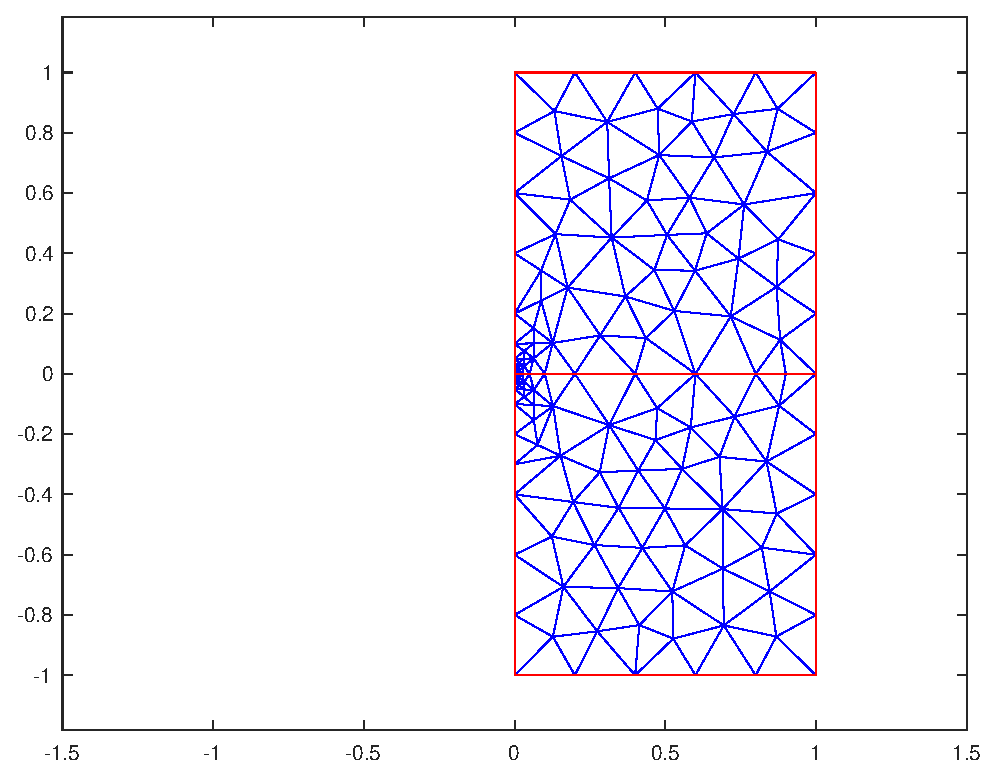
\includegraphics [width=4in]{lshape_neumann_meshsize2_07.eps}

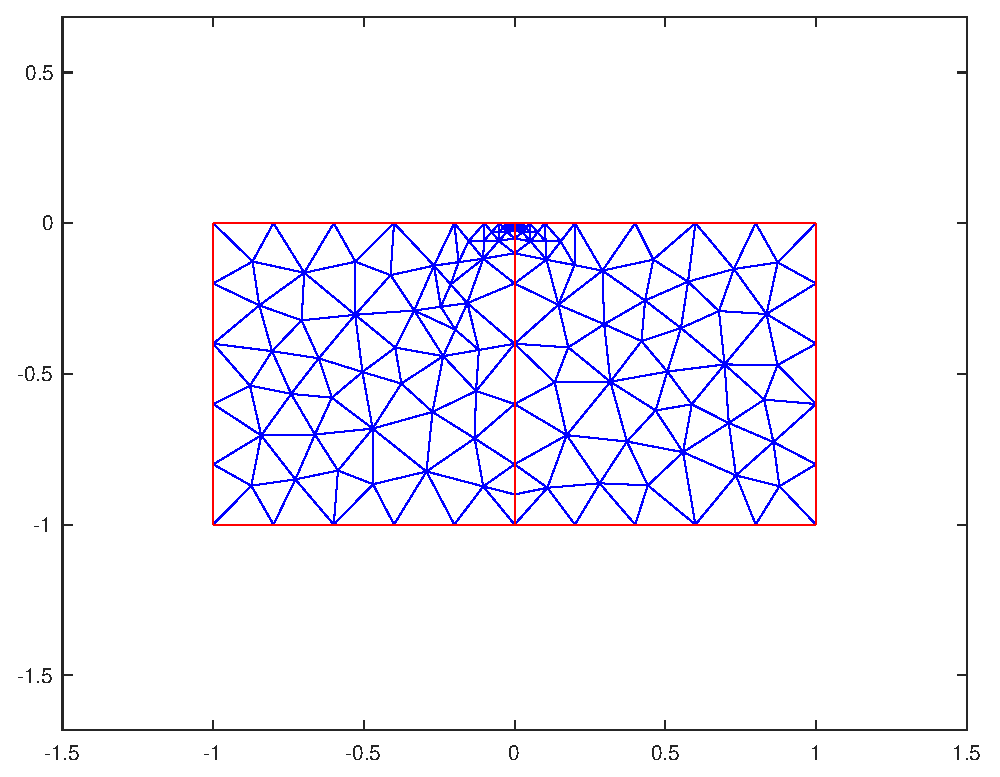
\includegraphics [width=4in]{lshape_neumann_meshsize2_08.eps}

\includegraphics [width=4in]{lshape_neumann_meshsize2_10.eps}

\includegraphics [width=4in]{lshape_neumann_meshsize2_11.eps}


\subsection*{Obtain relative matrices}

\begin{verbatim}
[K_up,M_up,F_up,Q_up,G_up,H_up,R_up]=assempde(b_up,p_up,e_up,t_up,c,a,f);
[K_lo,M_lo,F_lo,Q_lo,G_lo,H_lo,R_lo]=assempde(b_lo,p_lo,e_lo,t_lo,c,a,f);
\end{verbatim}


\subsection*{Assign true solution}

\begin{verbatim}
u_up_true = ones(1,length(p_up));
u_lo_true = ones(1,length(p_lo));
\end{verbatim}


\subsection*{Iterations}

\begin{verbatim}
counter = 0;
if rec == 1
    Vid = VideoWriter('Temp_video', 'MPEG-4');
    Vid.FrameRate = 3;
    Vid.Quality = 100;
    open(Vid);
end
ZZ(XX>=0) = initguess(XX(XX>=0),YY(XX>=0));
ZZ(YY<=0) = initguess(XX(YY<=0),YY(YY<=0));
figure(3);
my_plot_new(XX,YY,ZZ,az,el,v, plot_range, col_range,0,fix_axes);

if rec == 1
    frame = getframe(gcf);
    writeVideo(Vid,frame);
end
pause

% Note that pind_up2 represents the indices of the mesh points at the boundary in the
% upper domain
[pind_up1,pind_up2]=find(H_up);
% Remove the problematic point
ind=find((abs(p_up(1,pind_up2) -0)<1e-10) & (abs(p_up(2,pind_up2) -0)<1e-10));
pind_up1(ind)=[];
pind_up2(ind)=[];
% Update the Dirichlet condition matrix H_up
H_up=H_up(pind_up1,:);


[pind_lo1,pind_lo2]=find(H_lo);
% Remove the problematic point
ind=find((abs(p_lo(1,pind_lo2) -0)<1e-10) & (abs(p_lo(2,pind_lo2) -0)<1e-10));
pind_lo1(ind)=[];
pind_lo2(ind)=[];
% Update the Dirichlet condition matrix H_lo
H_lo=H_lo(pind_lo1,:);


bnew_up=zeros(length(pind_up2),1);
bnew_lo=zeros(length(pind_lo2),1);

for step = 1:Nsteps;
    if step == 1
        bfun_up = @(x,y) initguess(x,y);
    else
        bfun_up = @(x,y) tri2grid(p_lo,t_lo,u_lo,x,y);
    end
% Update  boundary conditions
for i=1:length(pind_up2);
    bnew_up(i)=bfun_up(p_up(1,pind_up2(i)),p_up(2,pind_up2(i)));
end
% Update the Dirichlet condtion vector R_up
 R_up = H_up(:,pind_up2)*bnew_up;

% Solve the pde in the upper domain
u_up=assempde(K_up,M_up,F_up,Q_up,G_up,H_up,R_up);

% Plot the solution
ZZ(XX>=0) = tri2grid(p_up,t_up,u_up,xg(indx_up),yg(indy_up));
figure(3);
my_plot_new(XX,YY,ZZ,az,el,v, plot_range, col_range, counter,fix_axes);

if rec == 1
    frame = getframe(gcf);
    writeVideo(Vid,frame);
end

pause(T)
counter = counter+1;

bfun_lo = @(x,y) tri2grid(p_up,t_up,u_up,x,y);

% Update the boundary conditions
for i=1:length(pind_lo2);
    bnew_lo(i)=bfun_lo(p_lo(1,pind_lo2(i)),p_lo(2,pind_lo2(i)));
end

% Update the Dirichlet condition vector
R_lo = H_lo(:,pind_lo2)*bnew_lo;

% Solve the pde in the lower domain
u_lo=assempde(K_lo,M_lo,F_lo,Q_lo,G_lo,H_lo,R_lo);

%Plot the solution
ZZ(YY<=0) = tri2grid(p_lo,t_lo,u_lo,xg(indx_lo),yg(indy_lo));
figure(3)
my_plot_new(XX,YY,ZZ,az,el, v, plot_range, col_range, counter,fix_axes);

if rec == 1
    frame = getframe(gcf);
    writeVideo(Vid,frame);
end

pause(T)

counter = counter+1;

% The error calculated with respect to infinity norm
errvals_inf(Nmesh/25,step)=max(max(abs([u_up(:); u_lo(:)]-[u_up_true(:); u_lo_true(:)])));

% The error calculated with respect to H1 norm

% The difference between the solution from ASM and the true solution
u_diff=ZZ-ones(size(ZZ));
% Square the difference
u_diff_square=u_diff.*u_diff;
%  stepsize on x-axis
dx=(1-(-1))/(Nplot-1);
% stepsize on y-axis
dy=(1-(-1))/(Nplot-1);
integral_1=sum(sum (dx*dy*u_diff_square(indices_all)));

% Approximate the derivatives by Central Difference Method
Du_dy=(ZZ(3:Nplot,:)-ZZ(1:Nplot-2,:))/(2*dy);
Du_dx=(ZZ(:,3:Nplot)-ZZ(:,1:Nplot-2))/(2*dx);
% Integrate on the y-direction
integrand_y=Du_dy.*Du_dy*dx*dy;
% Integrate on the x-direction
integrand_x=Du_dx.*Du_dx*dx*dy;
integrals=[integral_1,sum(sum(integrand_y(diffy_ind))),sum(sum(integrand_x(diffx_ind)))];
errvals_H1(Nmesh/25,step)=sqrt(sum(integrals));
end
\end{verbatim}

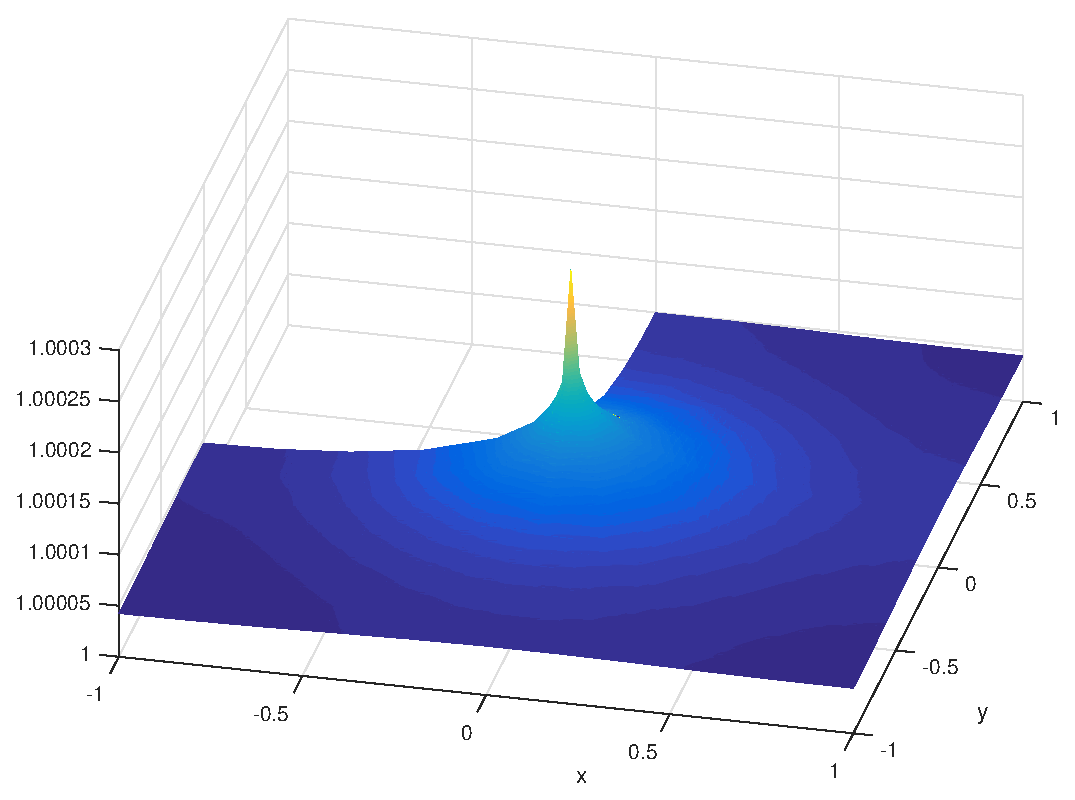
\includegraphics [width=4in]{lshape_neumann_meshsize2_03.eps}

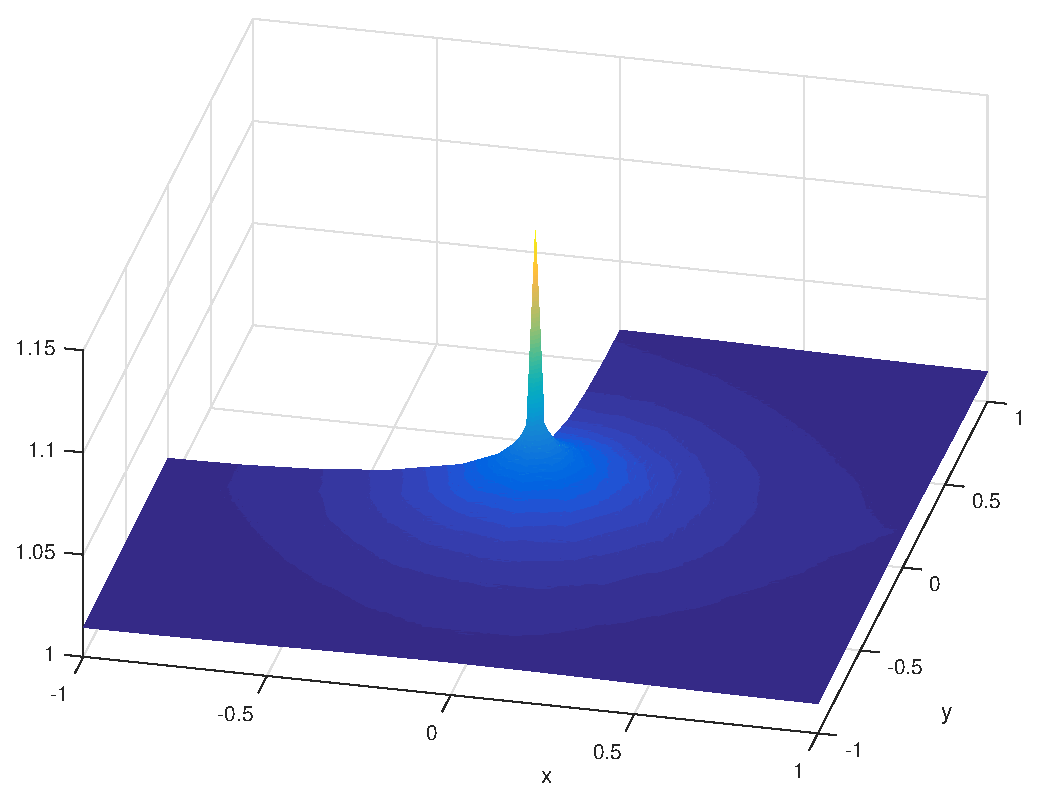
\includegraphics [width=4in]{lshape_neumann_meshsize2_06.eps}

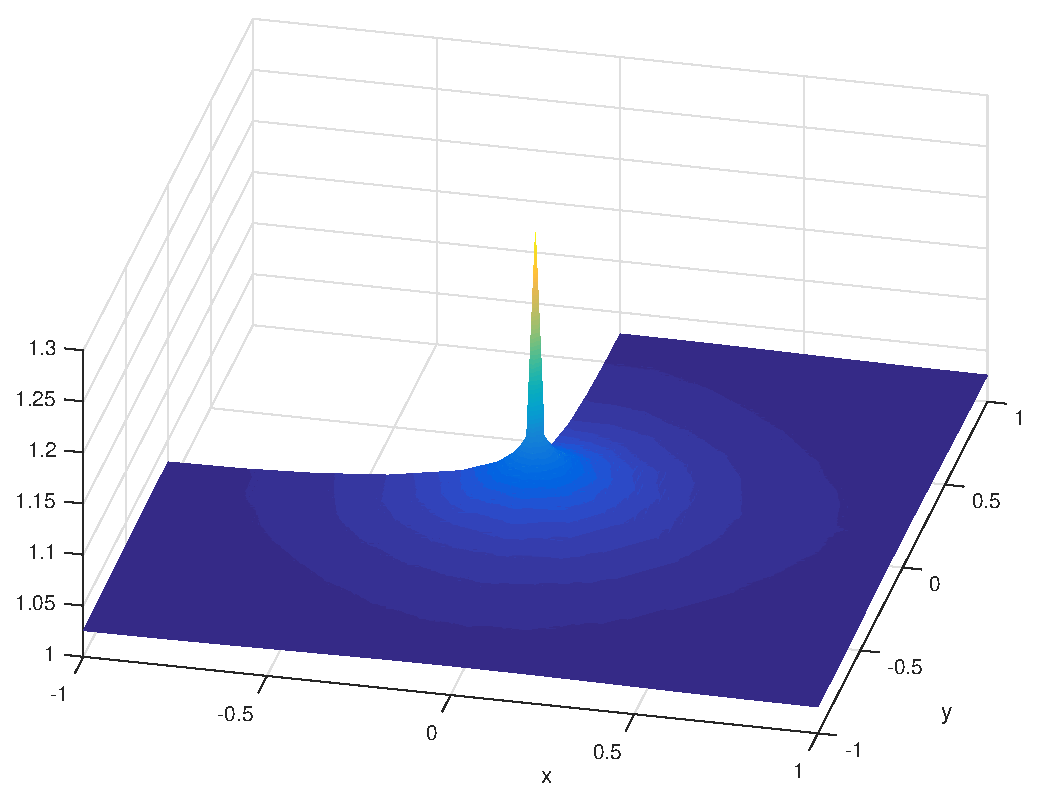
\includegraphics [width=4in]{lshape_neumann_meshsize2_09.eps}

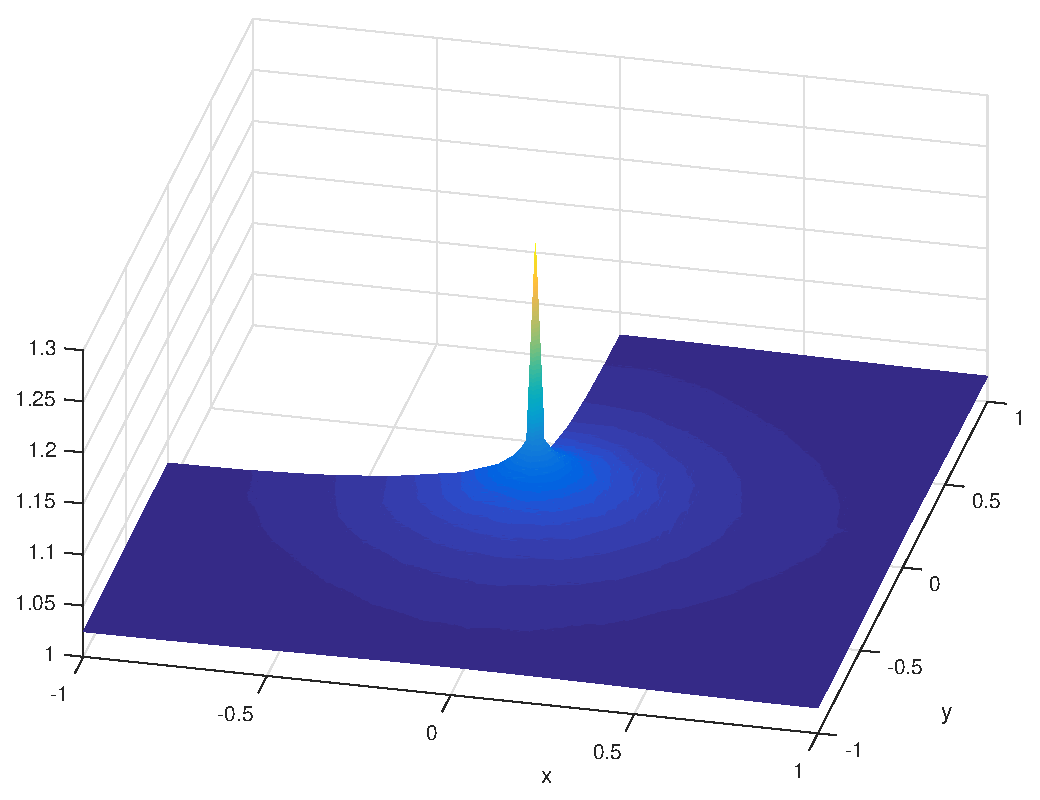
\includegraphics [width=4in]{lshape_neumann_meshsize2_12.eps}
\begin{verbatim}
end

if rec == 1
    close(Vid);
end
\end{verbatim}


\subsection*{Plot of \texttt{\ensuremath{|}u\_n-u\_true}\ensuremath{|} versus Nsteps}

\begin{verbatim}
figure(4)
nn = 1:Nsteps;
semilogy(nn,[errvals_inf(1,:);errvals_inf(2,:);errvals_inf(3,:);errvals_inf(4,:)]);
legend('Nmesh=25','Nmesh=50', 'Nmesh=75','Nmesh=100')
xlabel('Number of Iterations'); % x-axis label
ylabel('Log(errvals_{inf})') ;    % y-axis label

figure(5)
nn = 1:Nsteps;
semilogy(nn,[errvals_H1(1,:);errvals_H1(2,:);errvals_H1(3,:);errvals_H1(4,:)]);
legend('Nmesh=25','Nmesh=50', 'Nmesh=75','Nmesh=100');
xlabel('Number of Iterations'); % x-axis label
ylabel('Log(errvals_{H1})');     % y-axis label
toc
\end{verbatim}

        \color{lightgray} \begin{verbatim}Elapsed time is 90.622654 seconds.
\end{verbatim} \color{black}
    
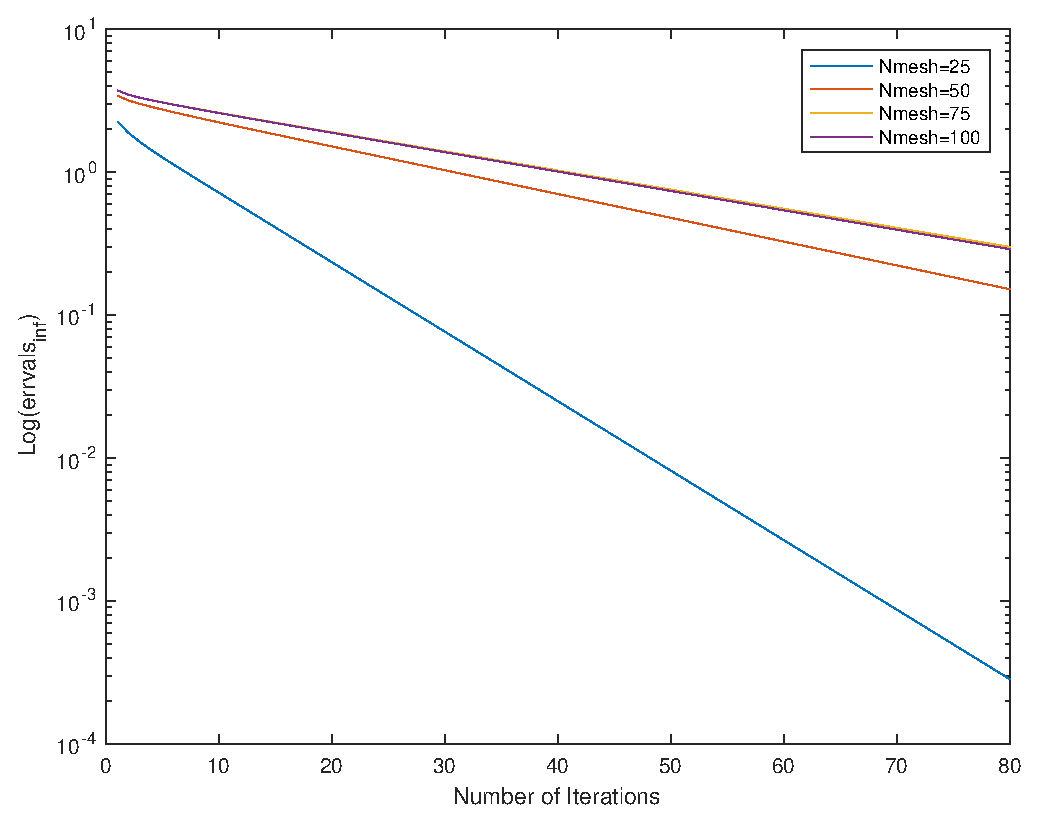
\includegraphics [width=4in]{lshape_neumann_meshsize2_13.eps}

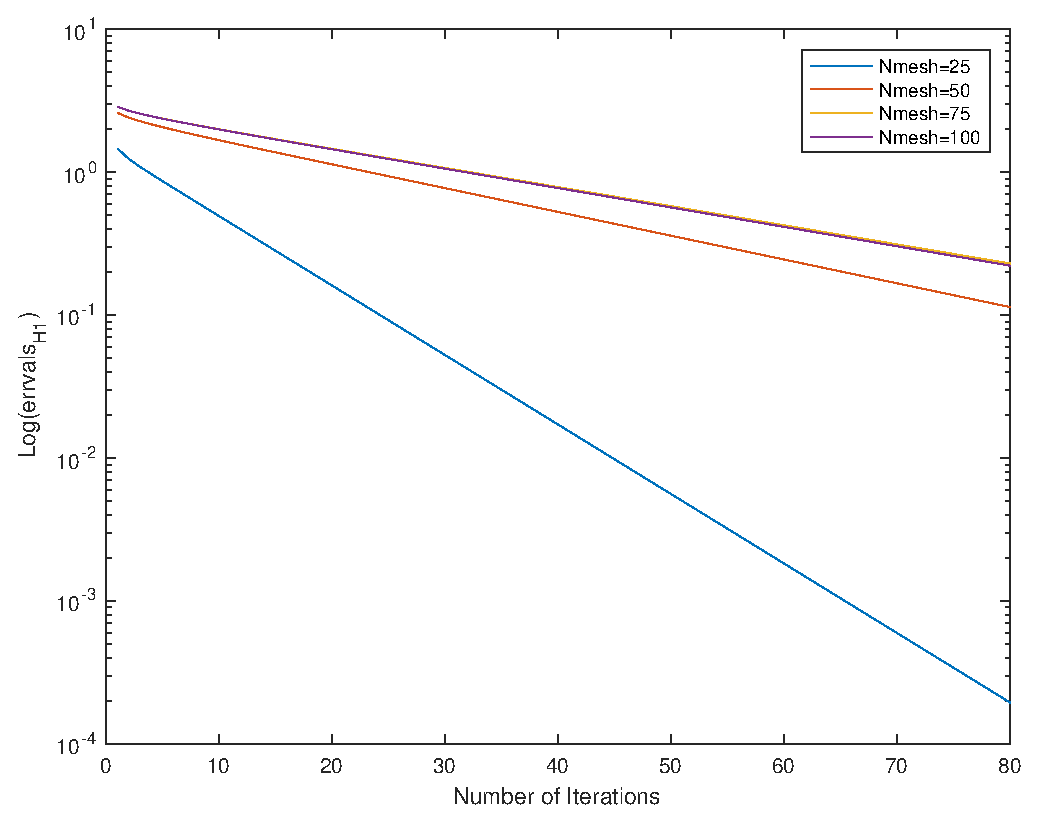
\includegraphics [width=4in]{lshape_neumann_meshsize2_14.eps}



\end{document}
    
